\section{Experimental setup}
\label{sec:experimental_design}

ICL is widely viewed as an emergent form of meta-learning. Accordingly, we use two standard benchmarks from the meta-learning literature: parametric sinusoid regression \cite{finn2017model} and few-shot Omniglot classification \cite{lake2015human}. These environments allow us to systematically manipulate our proposed dimensions of environmental predictability (cue reliability and environmental stability) across both continuous and discrete domains.

\subsection{Sinusoid regression}
\label{sec:experimental_design_sinusoid}

In the sinusoid regression task \cite{finn2017model}, the objective is to predict the output of a target function $f_t(x) = A_t \sin(x + \phi_t)$ (see Figure \ref{fig:sinusoid_task}). Each training episode consists of a prompt of $N=10$ examples, $\{(x_i, y_i)\}_{i=1}^N$, followed by a query input $x_q$ for which the model must predict the ground truth $y_q = f_t(x_q)$. The inputs $x$ are sampled uniformly from $[-\pi, \pi]$.

\begin{figure}[!ht]
  \centering
  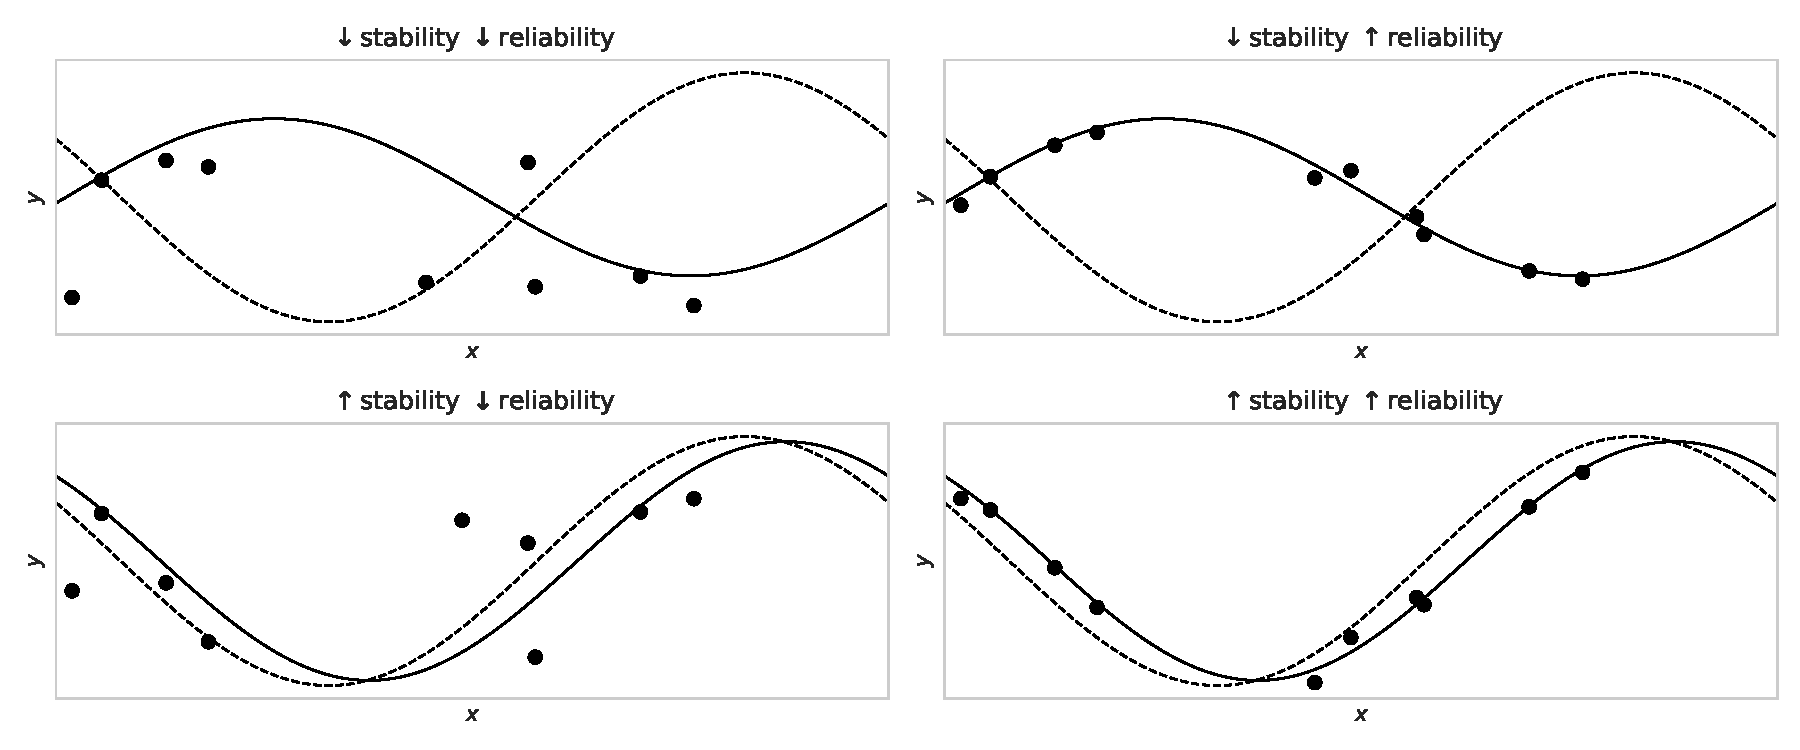
\includegraphics[width=0.99\linewidth]{figures/sinusoid_task.pdf}
  \caption{Sinusoid regression under varying predictability conditions. Each panel shows prompt examples (black dots) for a given target function at timestep $t$ (solid line), and the function at the preceding timestep $t-1$ (dashed line). Top row depicts volatile environments, meaning the target function changes significantly at each step. Bottom row depicts stable environments, where the target function is more stable across time. Left column depicts unreliable cues, where prompt examples are noisy. Right column depicts reliable cues, where prompt examples are less noisy and closer to the target function.}
  \label{fig:sinusoid_task}
\end{figure}

\textbf{Cue reliability.} We manipulate this by adjusting the variance, $\sigma^2$, of the Gaussian observation noise $\delta_i \sim \mathcal{N}(0, \sigma^2)$ added to the prompt targets $y_i$. A lower $\sigma^2$ corresponds to higher cue reliability, as the prompt examples more faithfully reflect the true underlying function $f_t$.

\textbf{Environmental stability.} We manipulate this by controlling the parameter $\alpha$ in an AR(1) process that governs the evolution of the task parameters $\theta_t = [A_t, \phi_t]^\top$ across training steps $t$. The parameter $\alpha \in [0, 1]$ dictates the correlation between successive tasks, where $\alpha \approx 1$ indicates high stability. The update rule is given by:

\begin{equation}
\theta_t = \alpha \theta_{t-1} + (1-\alpha)\tilde{\theta}_t
\label{eq:sinusoid_ar1}
\end{equation}

where $\tilde{\theta}_t$ represents random innovations drawn from the base task priors: amplitude $A \sim \mathcal{U}[0.5, 1.5]$ and phase $\phi \sim \mathcal{U}[0, 2\pi]$. This formulation ensures mean-reversion towards the prior distribution, allowing us to vary stability without drifting outside the solvable task distribution.

% In sinusoid regression \cite{finn2017model}, the task is to predict the output of a sinusoid function $f_t(x) = A_t \sin(x + \phi_t)$ (see Figure \ref{fig:sinusoid_task}). Each episode consists of prompt $N=10$ examples $\{(x_i, y_i)\}_{i=1}^N$ (inputs $x_i$ are sampled uniformly from $[-\pi, \pi]$, and corresponding outputs are $y_i = f_t(x_i) + \delta_i$, where $\delta_i$ represents Gaussian observation noise specific to each prompt example -- simulates cue reliability) and a query $x_q$ where the model must predict $y_q = f_t(x_q)$. The underlying function $f_t$ varies between episodes (timesteps $t$) -- simulates environmental volatility.

% The first task requires the model to perform regression on points sampled from a sinusoidal function (see Figure \ref{fig:sinusoid_task}), a setup inspired by prior meta-learning studies \cite{finn2017model}.

% Each training batch corresponds to a single environmental timestep $t$. Within a batch, all training sequences are generated from the same true underlying sinusoid $f_t(x) = A_t \sin(x + \phi_t)$. This setup mirrors a population adapting to a common, evolving environment.

% For each sequence, the model is provided with $N=10$ prompt examples $\{(x_i, y_i)\}_{i=1}^N$. Inputs $x_i$ are sampled uniformly from $[-\pi, \pi]$, and corresponding outputs are $y_i = f_t(x_i) + \delta_i$, where $\delta_i$ represents Gaussian observation noise specific to each prompt example. The model's objective is to predict the noise-free value $y_q = f_t(x_q)$ for a given query input $x_q$.

% \begin{figure}[!ht]
%   \centering
%   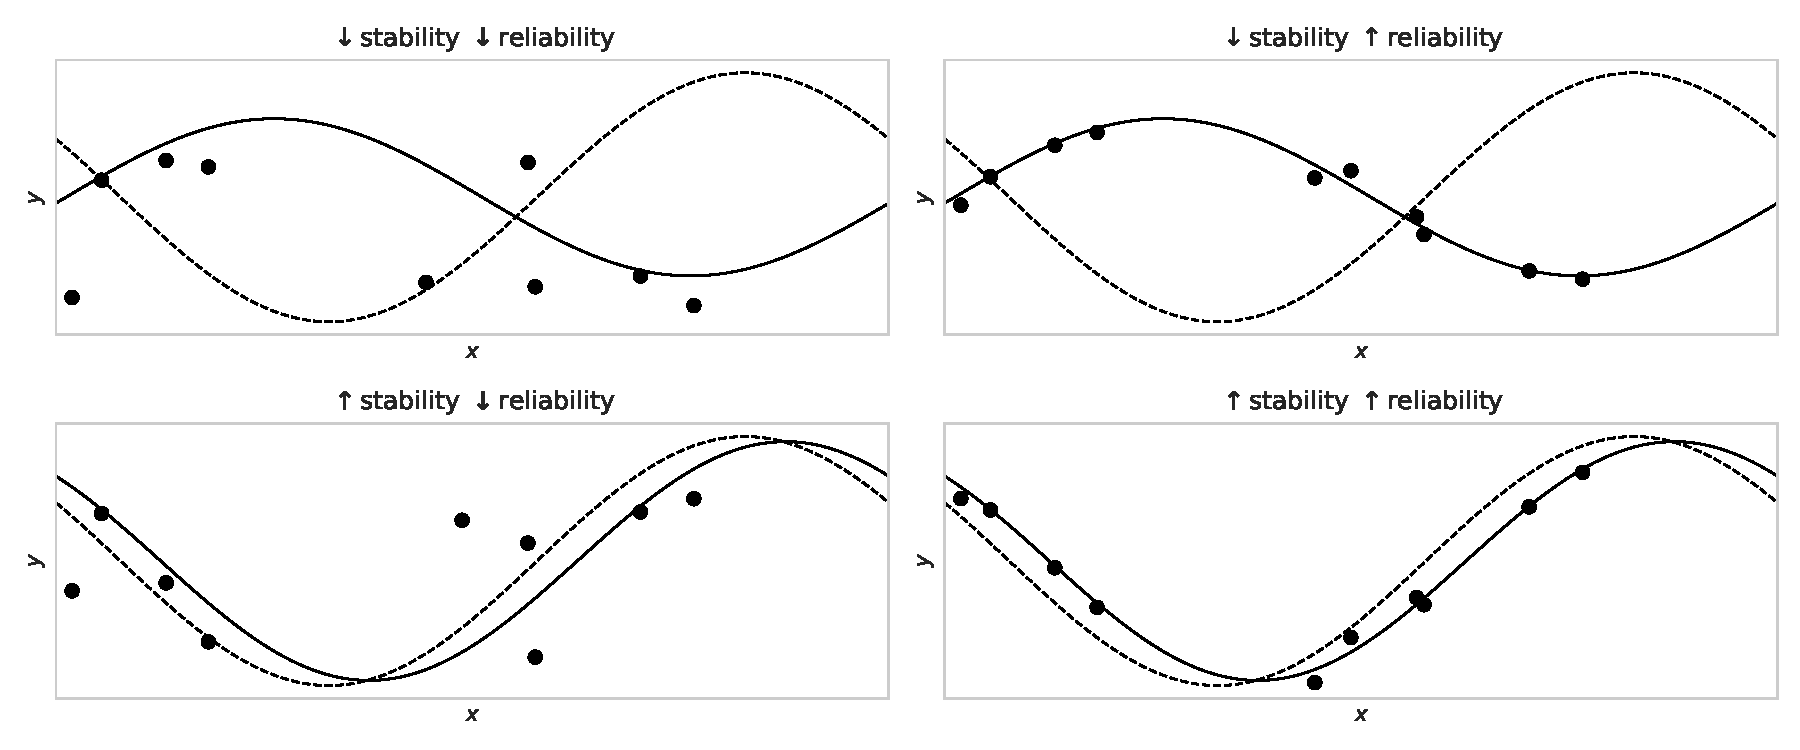
\includegraphics[width=0.99\linewidth]{figures/sinusoid_task.pdf}
%   \vspace{-0.5em}
%   \caption{Illustration of the sinusoid regression task under varying predictability conditions. Each panel shows prompt examples (black dots) for a given underlying sinusoid at timestep $t$ (solid line), and the sinusoid at the preceding timestep $t-1$ (dashed line). Top row: Low environmental stability, meaning the underlying sinusoid (solid line) changes significantly at each step. Bottom row: High environmental stability, where the underlying sinusoid is more stable across time. Left column: Low cue reliability, where prompt examples are noisy. Right column: High cue reliability, where prompt examples are less noisy and closer to the true underlying sinusoid.}
%   \label{fig:sinusoid_task}
% \end{figure}

% \textbf{Cue reliability.} This is manipulated by adjusting the variance, $\sigma^2_{\text{reliability}}$, of the Gaussian observation noise $\delta_i \sim \mathcal{N}(0, \sigma^2_{\text{reliability}})$ applied to the $y_i$ values in the prompt. Lower $\sigma^2_\text{reliability}$ corresponds to higher cue reliability.%, meaning prompt examples are more faithful to the true underlying sinusoid $f_t(x)$.

% \textbf{Environmental stability.} This is manipulated by controlling the parameter $\alpha_{\text{stability}}$ in an AR(1) process governing the evolution of the sinusoid parameters $\theta_t = [A_t, \phi_t]^T$ across successive environmental timesteps $t$. A higher $\alpha_{\text{stability}}$ indicates greater stability. The parameter update rule is:
% \begin{equation}
% \theta_t = \alpha_{\text{stability}} \theta_{t-1} + (1-\alpha_{\text{stability}})\theta_{\text{innovation}}^{(t)}
% \label{eq:sinusoid_ar1}
% \end{equation}
% where $\theta_0$ is initially sampled from prior distributions. For each subsequent timestep $t$, $\theta_{\text{innovation}}^{(t)}$ is a vector of innovations drawn afresh from these same priors:
% amplitude $A \sim U[0.5, 1.5]$ and phase $\phi \sim U[0, 2\pi]$. This formulation ensures mean-reversion towards the center of the prior distributions, with $\alpha_{\text{stability}}$ dictating the rate of change.

\subsection{Omniglot classification}

We adapt the few-shot Omniglot benchmark \cite{lake2015human} to construct a dynamic binary classification task (see Figure \ref{fig:omniglot_task}). At each training step $t$, a global mapping $M_t: \mathcal{C} \rightarrow \{0, 1\}$ assigns a hidden binary label to every character class $c$ in the Omniglot vocabulary $\mathcal{C}$ ($|\mathcal{C}| = 1623$). We define the target function $f_t(x) = M_t(c_x)$, where $c_x$ is the character class of image $x$.

Each episode consists of a prompt with $N=2$ image-label pairs $\{(x_i, y_i)\}_{i=1}^N$ and a query image $x_q$. The query image belongs to character class $c_q$, and the model must predict its current true label $M_t(c_q)$. Crucially, we construct the prompt such that one example matches the query's class ($c_k = c_q$). This setup explicitly creates a competition between strategies: the model can solve the task via ICL (copying the label $y_k$ from the matching prompt example) or via IWL (relying on the mapping $M_t(c_q)$ stored in its weights).

\begin{figure}[!ht]
  \centering
  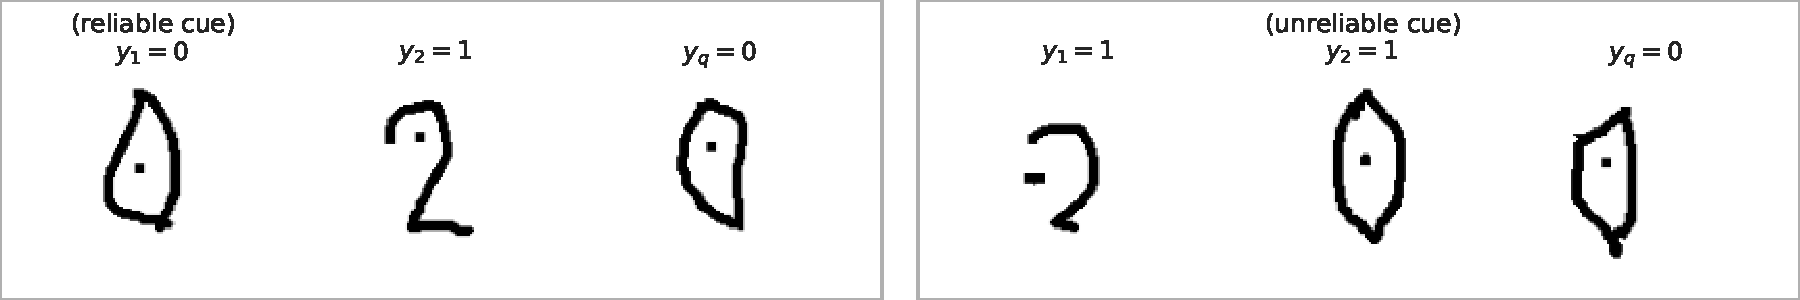
\includegraphics[width=0.99\linewidth]{figures/omniglot_task.pdf}
  \caption{Omniglot classification episodes. The prompt on the left contains a reliable cue (prompt label $y_1$ for character $c_1=c_q$ matches $M_t(c_q)$). The prompt on the right contains an unreliable cue (prompt label $y_2$ for $c_2=c_q$ is flipped relative to $M_t(c_q)$).}
  \label{fig:omniglot_task}
\end{figure}

\textbf{Cue reliability.} We operationalize reliability by controlling the probability, $\rho$, that prompt labels are accurate. For each example $i$ in the prompt, the provided label $y_i$ corresponds to the true mapping $M_t(c_i)$ with probability $\rho$, and is flipped otherwise:
\begin{equation}
y_i = \begin{cases} 
M_t(c_i) & \text{with probability } \rho \\
1 - M_t(c_i) & \text{with probability } 1 - \rho
\end{cases}
\label{eq:omniglot_reliability}
\end{equation}

\textbf{Environmental stability.} We operationalize stability by controlling the persistence of the global mapping $M_t$ over time. The initial mapping $M_0(c)$ is sampled from a Bernoulli(0.5) distribution. For subsequent steps $t > 0$, each character's label persists with probability $\gamma$:
\begin{equation}
M_t(c) = \begin{cases} 
M_{t-1}(c) & \text{with probability } \gamma \\
1 - M_{t-1}(c) & \text{with probability } 1 - \gamma
\end{cases}
\label{eq:omniglot_stability}
\end{equation}
A higher $\gamma$ indicates greater stability. This process induces a first-order temporal autocorrelation of $\alpha = 2\gamma - 1$ for each character's label trajectory.

% The second task is few-shot binary classification of Omniglot characters \cite{lake2015human} (see Figure \ref{fig:omniglot_task}). Similar to the sinusoid task, each training batch corresponds to a single environmental timestep t. At each timestep $t$, an underlying global mapping, $M_t: \mathcal{C} \rightarrow \{0, 1\}$, assigns a binary label to each character $c$ from a set $\mathcal{C}$ of 1623 unique Omniglot character classes.

% A prompt sequence comprises $N=2$ example image-label pairs $\{(x_i, y_i)\}_{i=1}^N$, followed by a query image $x_q$ (an exemplar of character class $c_q$). The model predicts the true binary label $M_t(c_q)$. Critically, one example character in the prompt, $c_k$, matches the query's class $c_k=c_q$. This allows the model to predict the query label by relying on the in-context label $y_k$ (ICL) or by accessing an internalized representation of $M_t(c_q)$ (IWL).

% \begin{figure}[!ht]
%   \centering
%   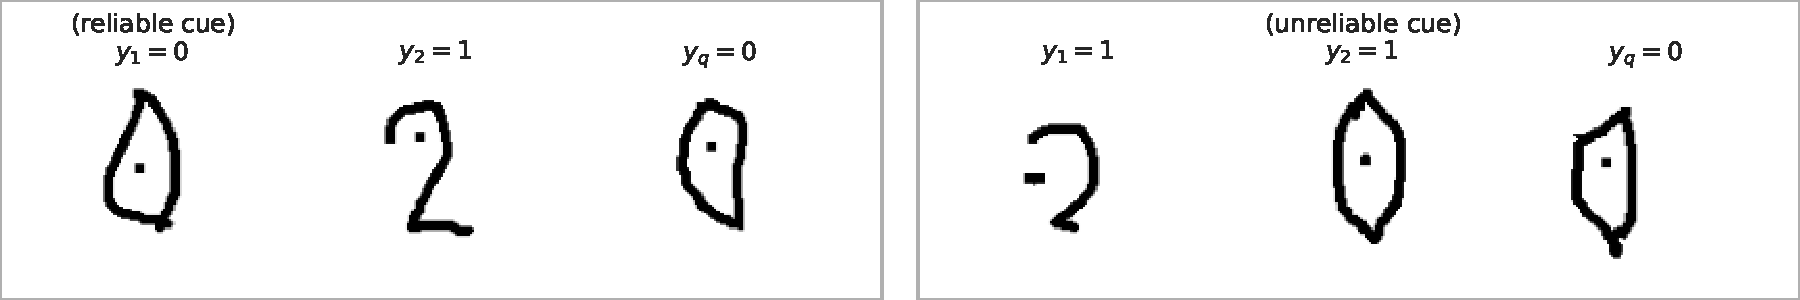
\includegraphics[width=0.99\linewidth]{figures/omniglot_task.pdf}
%   \vspace{-0.5em}
%   \caption{Sequences drawn from the Omniglot binary classification task. (\textbf{Left}) A sequence illustrating a reliable in-context cue (prompt label $y_1$ for character $c_1=c_q$ matches $M_t(c_q)$). (\textbf{Right}) A sequence illustrating an unreliable in-context cue (prompt label $y_2$ for $c_2=c_q$ is flipped relative to $M_t(c_q)$).}
%   \label{fig:omniglot_task}
% \end{figure}

% \textbf{Cue reliability.}
% This is manipulated by controlling the probability, $p_\text{reliability}$, that the label $y_i$ for a prompt character $c_i$ matches its true label $M_t(c_i)$. Specifically:
% \begin{equation}
% y_i = \begin{cases} 
% M_t(c_i) & \text{with probability } p_{\text{reliability}} \\
% 1 - M_t(c_i) & \text{with probability } 1 - p_{\text{reliability}}
% \end{cases}
% \label{eq:omniglot_reliability}
% \end{equation}
% Higher $p_\text{reliability}$ indicates higher cue reliability.

% \textbf{Environmental stability.}
% This is manipulated by varying the probability, $p$, that the true mapping $M_t(c)$ for each character $c$ persists from the previous timestep $M_{t-1}(c)$. The initial mapping $M_0(c)$ is sampled from Bernoulli(0.5) for all characters. For $t>0$:
% \begin{equation}
% M_t(c) = \begin{cases} 
% M_{t-1}(c) & \text{with probability } p \\
% 1 - M_{t-1}(c) & \text{with probability } 1 - p
% \end{cases}
% \label{eq:omniglot_stability}
% \end{equation}
% Higher $p_\text{stability}$ signifies greater environmental stability. The first-order temporal autocorrelation for each character's label in this process is 
% $\alpha=2p-1$.
% ranging from -1 (perfect anti-correlation if $p_\text{stability}=0$) to 1 (perfect stability if $p_\text{stability}=1$).

\subsection{Model and training}

% Drawing on the previous literature, we use both a sinusoid regression task \cite{finn2017model} and an Omniglot classification task \cite{lake2015human}.
All experiments use a decoder-only Transformer with 4 layers, 4 attention heads per layer, an embedding dimension of 128, and learned positional encodings.
Input processing varies by task. For the sinusoid regression task, scalar inputs and outputs are linearly projected to the embedding dimension. For Omniglot classification, character images are processed by a shallow ResNet with three stages, each with 2 residual blocks, and outputting 16, 32, and 64 channels per stage, respectively. This ResNet is trained jointly with the Transformer.

Models are optimized to minimize either the mean squared error (MSE) for sinusoid regression or the binary cross-entropy (BCE) for Omniglot classification, calculated on their predictions for the query item ($y_q$). We use the AdamW optimizer \cite{loshchilov2017decoupled} with a peak learning rate of $1 \times 10^{-4}$, subject to a cosine decay schedule following 1,000 warmup steps. All models are trained for a total of 50,000 training steps, using a batch size of 128.

\subsection{Evaluation}

To quantify the model's preference for ICL versus IWL, we use an evaluation protocol inspired by \citet{chan2022data}. This involves constructing evaluation prompts where the underlying target task explicitly conflicts with the current training environment.

\textbf{Evaluation prompts.} We generate these prompts by sampling an evaluation task, $f_e$, from the prior distribution such that it is independent of the current training task, $f_t$. We then construct a prompt $\{(x_i, y_i)\}_{i=1}^N$ using labels derived from this evaluation task ($y_i = f_e(x_i)$).

\textbf{Target definitions.} For a given query $x_q$, this setup defines two conflicting prediction targets:
\begin{itemize}
    \item The ICL target, $y_\text{ICL}=f_e(x_q)$, corresponds to the label implied by the prompt; a model predicting this value is relying on context (ICL).
    \item The IWL target, $y_\text{IWL}=f_t(x_q)$, corresponds to the label implied by the current training environment; a model predicting this value disregards the prompt in favor of its weight-based encoding of the environment (IWL).
\end{itemize}

\textbf{Quantifying strategy preference.} We quantify the model's strategy preference by computing the prediction error relative to both targets ($E_\text{ICL}$ and $E_\text{IWL}$) using the task-appropriate metric (MSE for Sinusoid, BCE for Omniglot). We define the ICL preference score as:
\begin{equation}S_\text{ICL} = \frac{E_\text{IWL}}{E_\text{ICL} + E_\text{IWL}}\label{eq:s_icl_preference}\end{equation}
An $S_\text{ICL} \approx 1$ indicates pure reliance on context, while $S_\text{ICL} \approx 0$ indicates pure reliance on weights.
% This metric captures strategy preference, not absolute task performance.

% To assess a trained model's preference for ICL versus IWL solutions, we employ a targeted evaluation protocol inspired by prior work \cite{chan2022data}. This evaluation is performed periodically during training. It uses novel evaluator tasks sampled from the same prior distributions as the training tasks but unseen during training. This allows us to contrast mappings learned in weights against those learnable from context during evaluation.

% \textbf{Evaluator tasks.} 
% For sinusoid regression, an evaluator task is a specific function $f_e(x) = A_e \sin(x + \phi_e)$ with $(A_e, \phi_e)$ newly sampled from their priors (Section \ref{sec:experimental_design_sinusoid}).
% For Omniglot classification, an evaluator task is a complete binary mapping $M_e: \mathcal{C} \rightarrow \{0, 1\}$ where each $M_e(c)$ is independently sampled from Bernoulli(0.5).
% For each evaluator task ($f_e$ or $M_e$) and a query input $x_q$, we construct a noiseless evaluation prompt $P_e = \{(x_j, y_j)\}_{j=1}^{N}$, with examples derived directly from $f_e$ or $M_e$. For Omniglot, one example in $P_e$ matches $c_q$. The model then predicts $\hat{y}_q$ (sinusoid) or $\hat{p}_q = P(y_q=1 | P_e, x_q)$ (Omniglot).

% \textbf{Evaluator targets.}
% At the moment of periodic evaluation, we define two conflicting targets for the model's prediction:
% \begin{itemize}
%     \item \textbf{ICL target:} The ground-truth for $x_q$ from the current evaluator task: $f_e(x_q)$ or $M_e(c_q)$. This target is independent of the training environment's state.
%     \item \textbf{IWL target}: The ground-truth for $x_q$ from the current state of the training environment generator (i.e., $f_t(x_q)$ or $M_t(c_q)$ at the time of evaluation). This reflects what a model relying purely on an internalized representation of the latest training environment state would predict.
% \end{itemize}

% \textbf{Quantifying preference.}
% We calculate the model's prediction error relative to both targets ($E_\text{ICL}$ and $E_\text{IWL}$) using mean squared error (sinusoid) or binary cross-entropy (Omniglot). A model prefers ICL if $E_\text{ICL} > E_\text{IWL}$. We quantify this preference using the score:
% \begin{equation}
%     S_\text{ICL} = \frac{E_\text{IWL}}{E_\text{ICL} + E_\text{IWL} + \epsilon}
% \label{eq:s_icl_preference}
% \end{equation}
% where $\epsilon$ (e.g., $1 \times 10^{-8}$) ensures numerical stability. $S_\text{ICL} > 0.5$ indicates ICL preference. This metric captures strategy preference, not absolute task performance.

% Further details and standard performance metrics are in the appendix.
